\documentclass{beamer}
\usepackage{tikz}
\usepackage[all]{xy}
\usepackage{amsmath,amssymb}
\usepackage{hyperref}
\usepackage{graphicx}
\usepackage{algorithmic}
\usepackage{multirow}

\DeclareMathOperator*{\argmin}{arg\,min}
\DeclareMathOperator*{\Lik}{Lik}
\DeclareMathOperator*{\PoissonLoss}{PoissonLoss}
\DeclareMathOperator*{\Peaks}{Peaks}
\DeclareMathOperator*{\Segments}{Segments}
\DeclareMathOperator*{\argmax}{arg\,max}
\DeclareMathOperator*{\maximize}{maximize}
\DeclareMathOperator*{\minimize}{minimize}
\newcommand{\sign}{\operatorname{sign}}
\newcommand{\RR}{\mathbb R}
\newcommand{\ZZ}{\mathbb Z}
\newcommand{\NN}{\mathbb N}
\newcommand{\z}{$z = 2, 4, 3, 5, 1$} 

\newcommand{\algo}[1]{\textcolor{#1}{#1}}
\definecolor{PDPA}{HTML}{66C2A5}
\definecolor{CDPA}{HTML}{FC8D62}
\definecolor{GPDPA}{HTML}{4D4D4D}

% Set transparency of non-highlighted sections in the table of
% contents slide.
\setbeamertemplate{section in toc shaded}[default][100]
\AtBeginSection[]
{
  \setbeamercolor{section in toc}{fg=red} 
  \setbeamercolor{section in toc shaded}{fg=black} 
  \begin{frame}
    \tableofcontents[currentsection]
  \end{frame}
}

\begin{document}

\title{Introduction to machine learning and neural networks}

\author{
  Toby Dylan Hocking\\
  toby.hocking@nau.edu\\
  toby.hocking@r-project.org\\
}

\maketitle

\section{Introduction and applications}

\begin{frame}
  \frametitle{Machine learning intro: image classification example}
  ML is all about learning predictive functions $f(x)\approx y$, where 
  \begin{itemize}
  \item Inputs/features $x$ can be easily computed using traditional
    algorithms, e.g. matrix of pixel intensities in an image.
  \item Outputs/labels $y$ are what we want to predict, easy to get by
    asking a human, but hard to compute using traditional algorithms,
    e.g. image class.
  \item Input $x$ = image of digit, output $y\in\{0,1,\dots,9\}$, \\--
    this is a classification problem with 10 classes.\\
  $f(
\includegraphics[height=1cm]{mnist-0})=0$,
  $f(
\includegraphics[height=1cm]{mnist-1})=1$
\item Traditional/unsupervised algorithm: I give you a pixel intensity matrix
  $x\in\RR^{16\times 16}$, you code a function $f$ that returns one of
  the 10 possible digits. Q: how to do that?
  \end{itemize}
\end{frame}

\begin{frame}
  \frametitle{Supervised machine learning algorithms}

  I give you a training data set with paired inputs/outputs, e.g.

  \begin{center}
    \Huge 0 1 2 3 4 5 6 7 8 9

  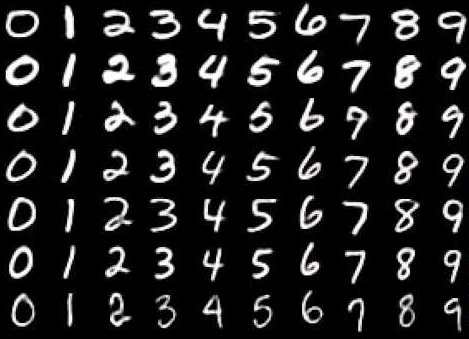
\includegraphics[height=1.9in]{mnist-digits}
  \end{center}

  Your job is to code an algorithm that learns the function $f$ from
  the training data. (you don't code $f$)
  
  \scriptsize Source: github.com/cazala/mnist
\end{frame}


\begin{frame}
  \frametitle{Advantages of supervised machine learning}

  \begin{center}
      \begin{tabular}{cc}
        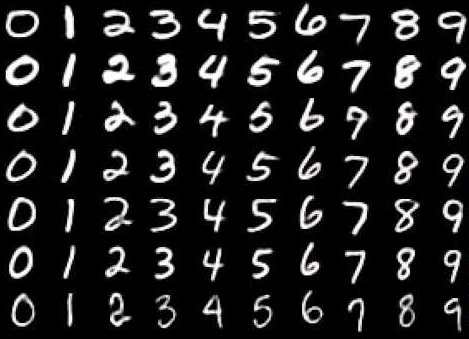
\includegraphics[height=1.5in]{mnist-digits} &
  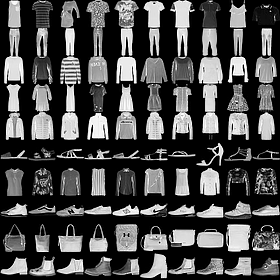
\includegraphics[height=1.5in]{fashion-mnist-sprite-some}  
  \end{tabular}
  \end{center}
  \vskip -0.2cm
  
  \begin{itemize}
  \item Input $x\in\RR^{16\times 16}$, output $y\in\{0,1,\dots,9\}$ types the same!
  \item Can use same learning algorithm regardless of pattern.
  \item Pattern encoded in the labels (not the algorithm).
  \item Useful if there are many un-labeled data, but few labeled data
    (or getting labels is long/costly).
  \item State-of-the-art accuracy (if there is enough training data).
  \end{itemize}

  \scriptsize Sources: github.com/cazala/mnist, github.com/zalandoresearch/fashion-mnist

\end{frame}

\begin{frame}
  \frametitle{Learning two different functions}
  Say \textsc{Learn} is a learning algorithm you have coded.
  \begin{center}
      \begin{tabular}{c}
        \textsc{Learn}(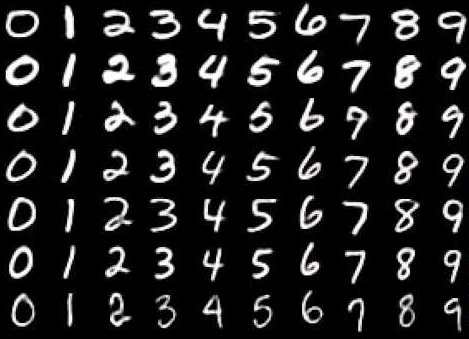
\includegraphics[height=1in]{mnist-digits}) $\rightarrow f$, 
        \textsc{Learn}(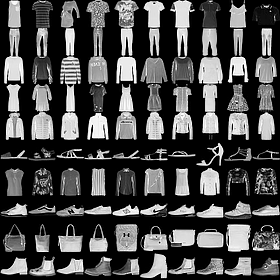
\includegraphics[height=1in]{fashion-mnist-sprite-some}) $\rightarrow g$
  \end{tabular}
  \end{center}
  \begin{itemize}
  \item Then we would expect
    $f(
\includegraphics[height=1cm]{mnist-0})=0$,
    $f(
\includegraphics[height=1cm]{mnist-1})=1$
  \item $g(
\includegraphics[height=1cm]{fashion-mnist-boot})=\text{shoe/0}$,
  $g(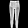
\includegraphics[height=1cm]{fashion-mnist-pants})=\text{pants/1}$
  \item Q: what happens if you do 
    $f(
\includegraphics[height=1cm]{fashion-mnist-boot})$, or
   $g(
\includegraphics[height=1cm]{mnist-0})$?

  \end{itemize}
\end{frame}

\begin{frame}
  \frametitle{Machine learning for cell image classification (CellProfiler)}
  Jones {\it et al.} PNAS 2009. Scoring diverse cellular morphologies in
  image-based screens with iterative feedback and machine learning.

\parbox{2in}{
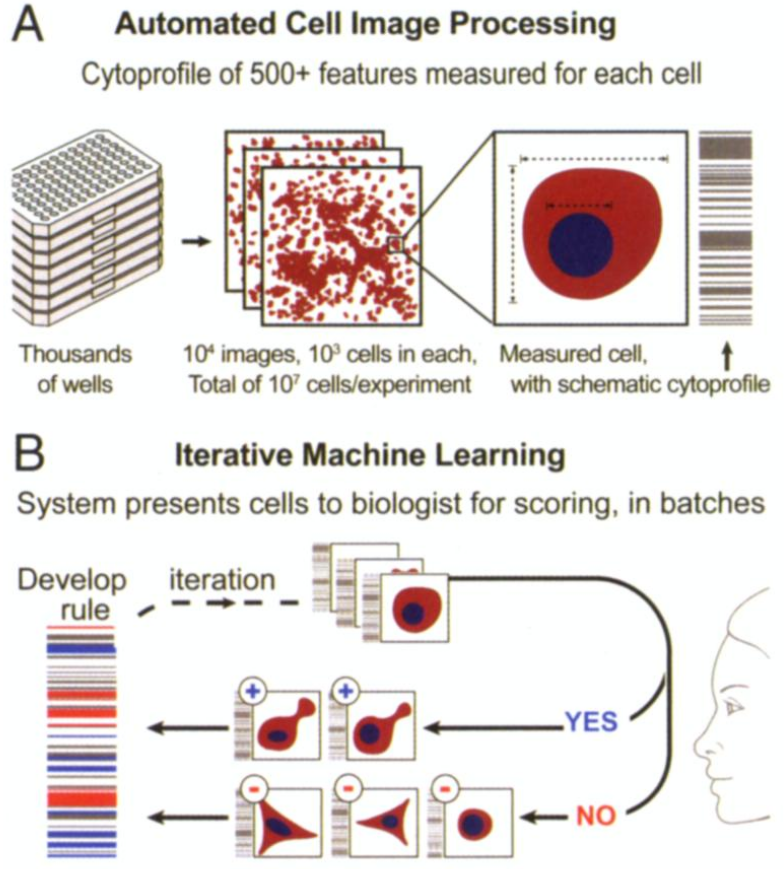
\includegraphics[width=2in]{cellprofiler} 
}
\parbox{2in}{
\begin{itemize}
  \item Input $x$ = image of cell, 
  \item Output $y\in\{\text{yes}, \text{no}\}$ (binary classification),
  \item $f(
\includegraphics[height=1cm]{cellprofiler-yes})=\text{yes}$,
  \item $f(
\includegraphics[height=1cm]{cellprofiler-no})=\text{no}$.
  \end{itemize}
}
\end{frame}

\begin{frame}
  \frametitle{Machine learning for image segmentation (LabelMe)}

  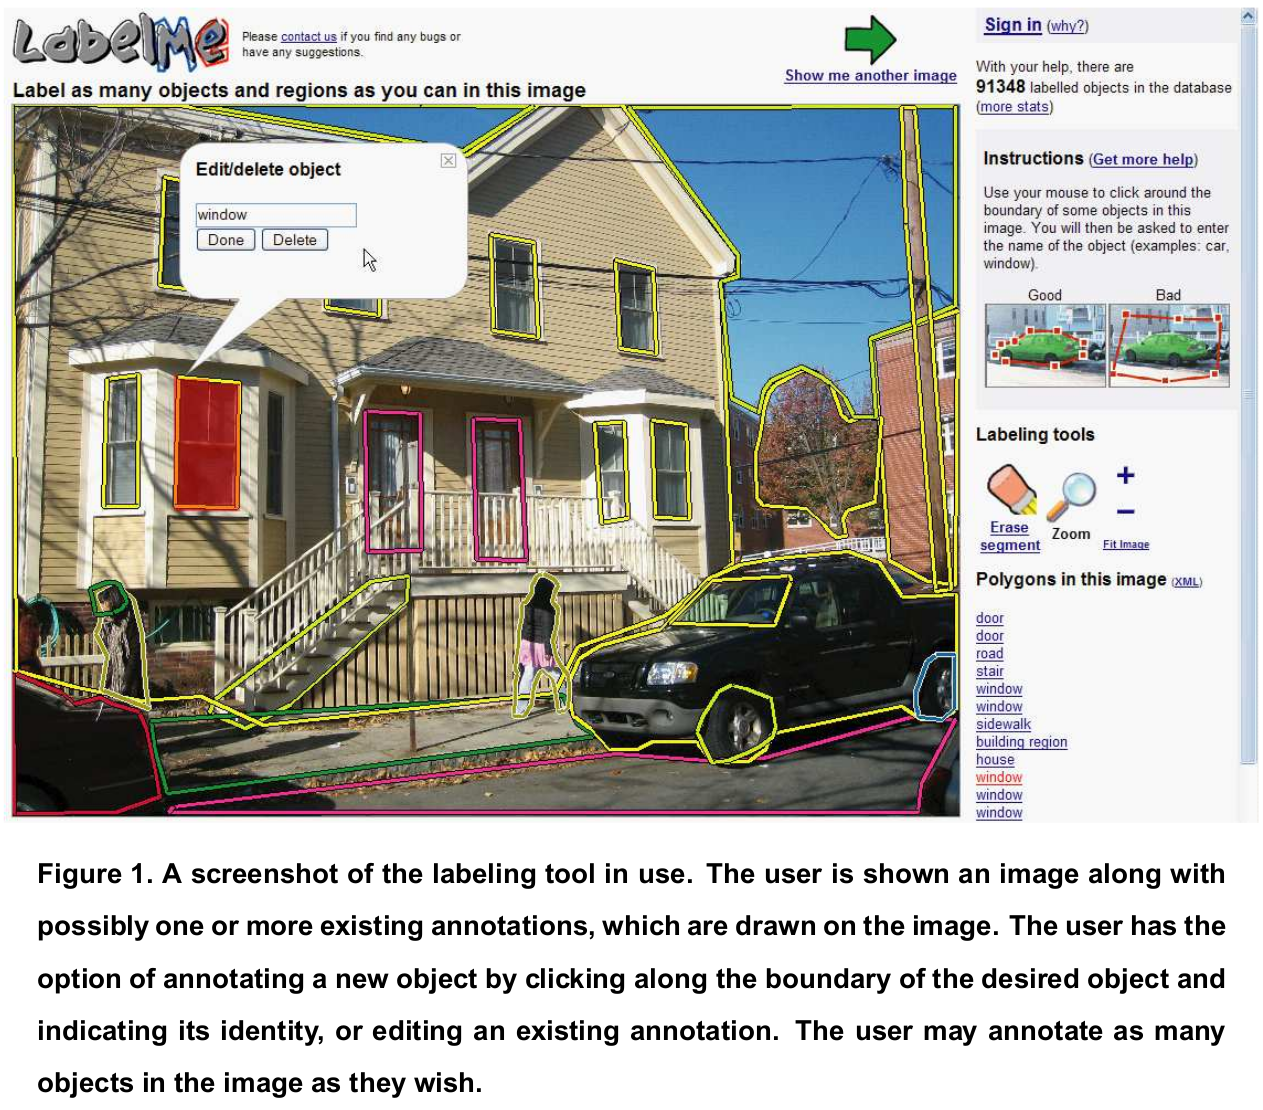
\includegraphics[width=\textwidth]{image-segmentation/labelme-interface}

\end{frame}

\begin{frame}
  \frametitle{Machine learning for image segmentation}

  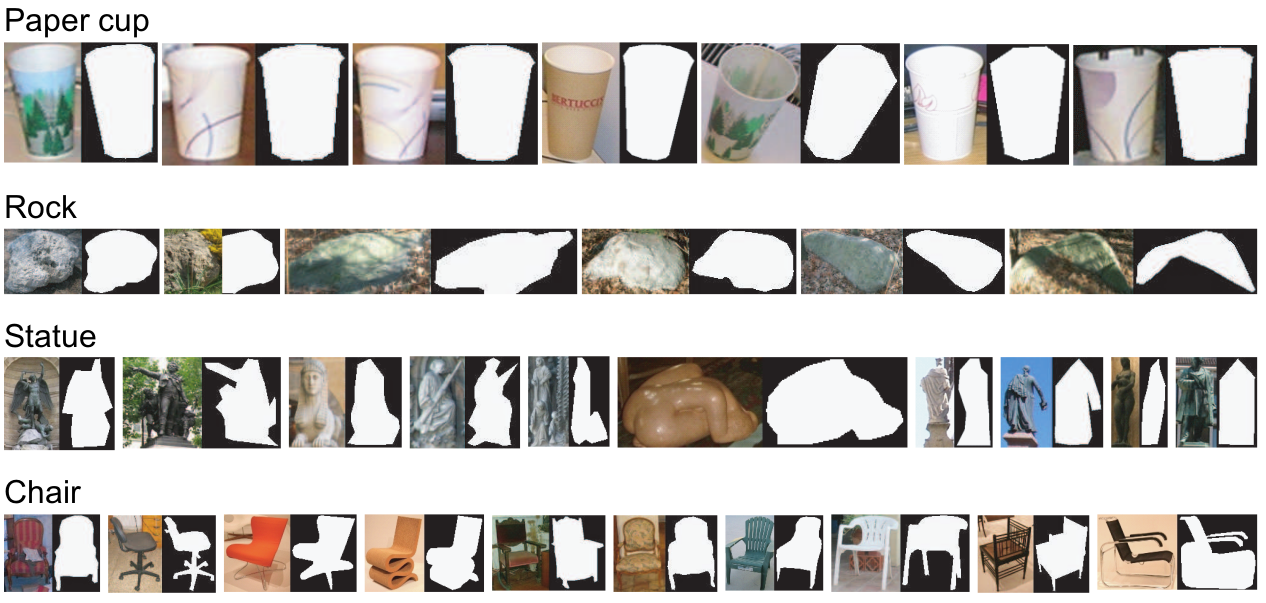
\includegraphics[width=\textwidth]{image-segmentation/labelme-examples}

  Russell {\it et al.} 2007.

  Q: What are the types/dimensions of $x,y,f$ in this example?

\end{frame}



\begin{frame}
  \frametitle{Machine learning for spam filtering (Gmail)}

  
\includegraphics[height=2in]{spam-filtering/screenshot-gmail-spam}
  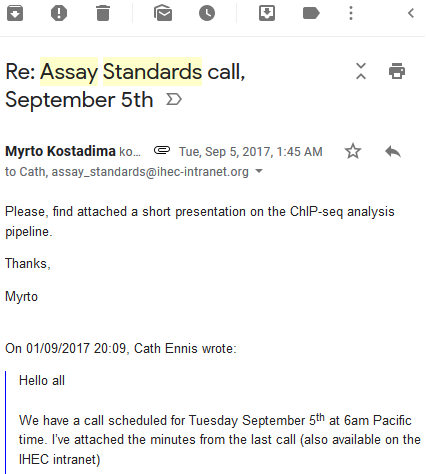
\includegraphics[height=2in]{spam-filtering/screenshot-inbox-message}

  Want: $f$(email message)$\in\{0,1\}$ -- binary classification, spam=1
  or not=0.

\end{frame}


\begin{frame}
  \frametitle{Machine learning for translation (google books)}

  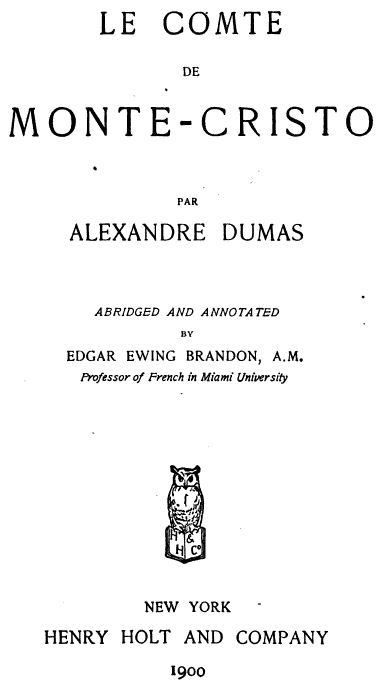
\includegraphics[height=3in]{translation/monte-cristo-french-title}
  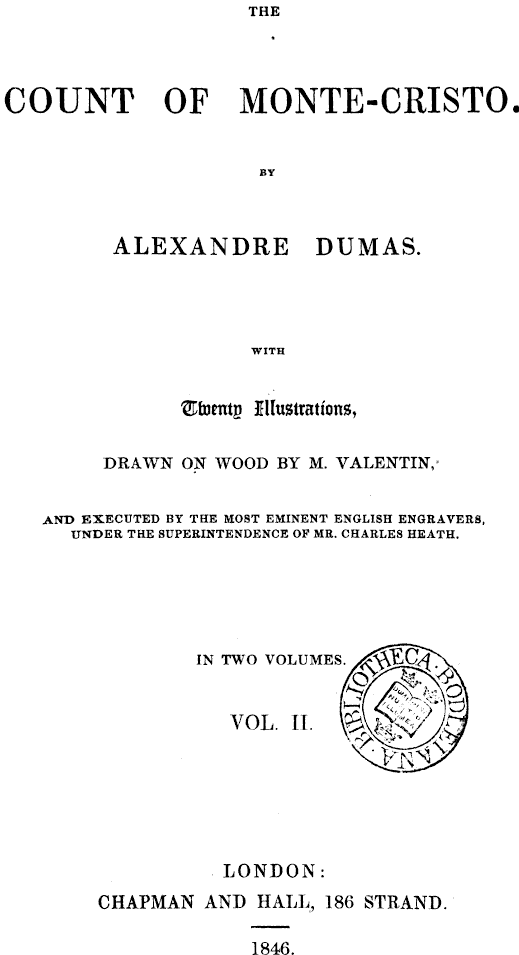
\includegraphics[height=3in]{translation/monte-cristo-english-title}

\end{frame}

\begin{frame}
  \frametitle{Machine learning for translation (google translate)}

  
  Want: $f$(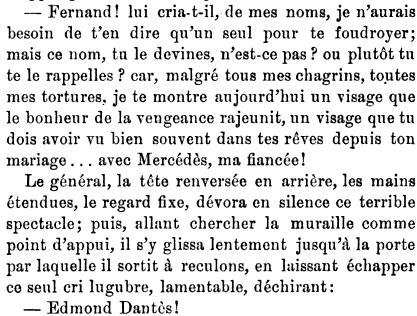
\includegraphics[width=0.5\textwidth]{translation/monte-cristo-french}) =
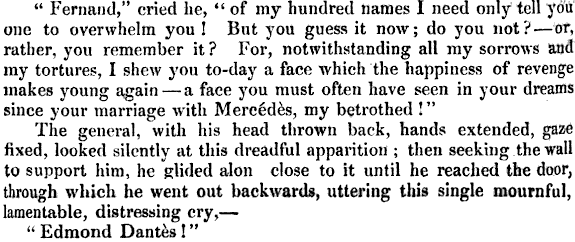
\includegraphics[width=0.8\textwidth]{translation/monte-cristo-english}

\end{frame}

\begin{frame}
  \frametitle{Machine learning for medical diagnosis}

\parbox{0.49\textwidth}{
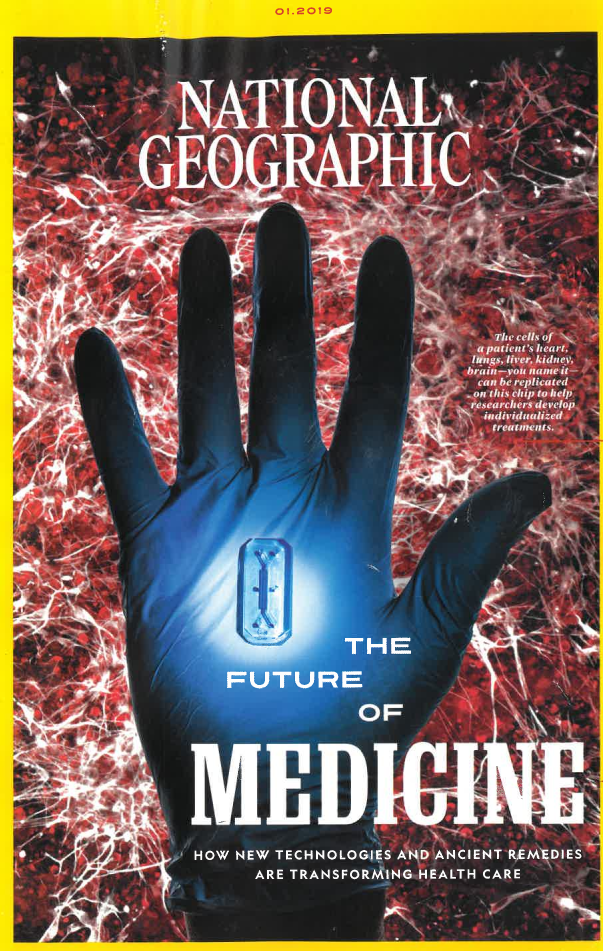
\includegraphics[height=0.9\textheight]{retinal-scans/national-geographic-medicine-cover}
}
\parbox{0.49\textwidth}{
f(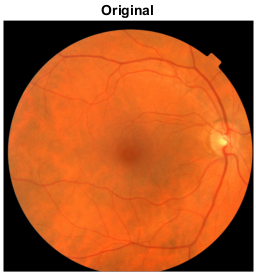
\includegraphics[width=0.5\textwidth]{retinal-scans/national-geographic-medicine-retina})=
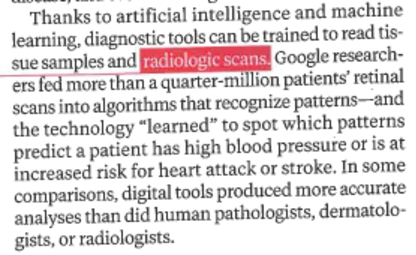
\includegraphics[width=0.5\textwidth]{retinal-scans/national-geographic-medicine-paragraph})
}

\end{frame}

\section{Practical considerations}

\begin{frame}
  \frametitle{Machine learning algorithms in practice}

  To learn a good prediction function for any of these problems (and
  any other problems you encounter in your work) you should
  \begin{itemize}
  \item First gather a data set that you will use to train/test the
    machine learning algorithms, typically a CSV file with rows for
    observations and columns for features.
  \item Use K-fold Cross-Validation to repeatedly divide the
    observations into train/test sets. Use the train set to learn
    machine learning model parameters, and use the test set to
    estimate prediction error.
  \item Try a variety of different learning algorithms (e.g. linear
    models, random forests, boosting, neural networks, support vector
    machines, ...), because you don't know which one will result in
    most accurate predictions for any given data set. 
  \item Each learning algorithm has different hyper-parameters which
    control complexity/regularization/overfitting, and typically must
    be chosen by the user (you) by dividing the train data into
    subtrain/validation sets. Use the hyper-parameter which is
    best with respect to the held-out validation set.
  \end{itemize}
  
\end{frame}

\begin{frame}
  \frametitle{Creating/reading CSV data tables}
  \begin{itemize}
  \item One row for each observation.
  \item One column for the output/label (in regression the label is a real
    number, in classification the label is a class/category).
  \item The other columns should be inputs/features that will be used
    to predict the corresponding output/label.
  \end{itemize}

  Examples:
  \begin{itemize}
  \item TODO
  \end{itemize}
\end{frame}

\begin{frame}[fragile]
  \frametitle{K-fold cross-validation for evaluating prediction accuracy}
  Randomly create a vector of fold ID numbers from 1 to K, one fold ID
  for each observation:

\begin{verbatim}
set.seed(1) #for reproducibility.
n.folds <- 4
unique.folds <- 1:n.folds
fold.vec <- sample(rep(unique.folds, l=N.observations))
\end{verbatim}

  The results:

\begin{verbatim}
> unique.folds
[1] 1 2 3 4
> str(fold.vec)
 int [1:100] 4 3 1 2 3 3 2 2 3 3 ...
\end{verbatim}
  
\end{frame}

\begin{frame}
  \frametitle{Hyper-parameter tuning}
  Fix a hyper-parameter value and use the
    subtrain data to fit use the subtrain data to learn a model for
    each of hyper-parameters, then use the hyper-parameters that
    result in maximal prediction accuracy with respect to the .
\end{frame}

% QUIZ 1. purpose of train/subtrain/validation/test
% sets. 2. overfitting/underfitting. 3. data input format for
% ML. 4. cross-validation fold ID / test/train sets.

\section{Demonstration of overfitting in regression}

\begin{frame}
  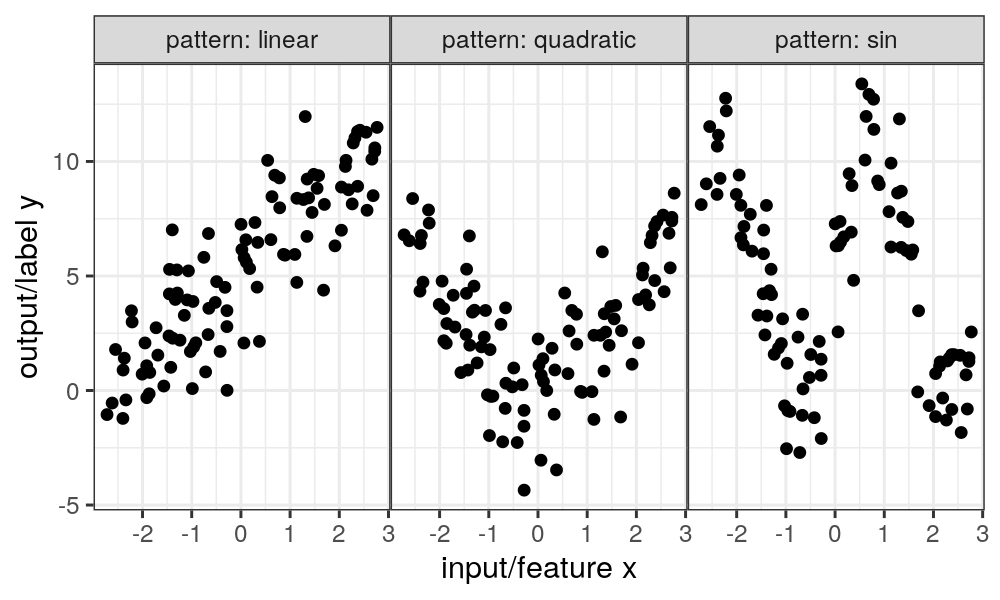
\includegraphics[width=\textwidth]{figure-overfitting-data}
\end{frame}

\begin{frame}
  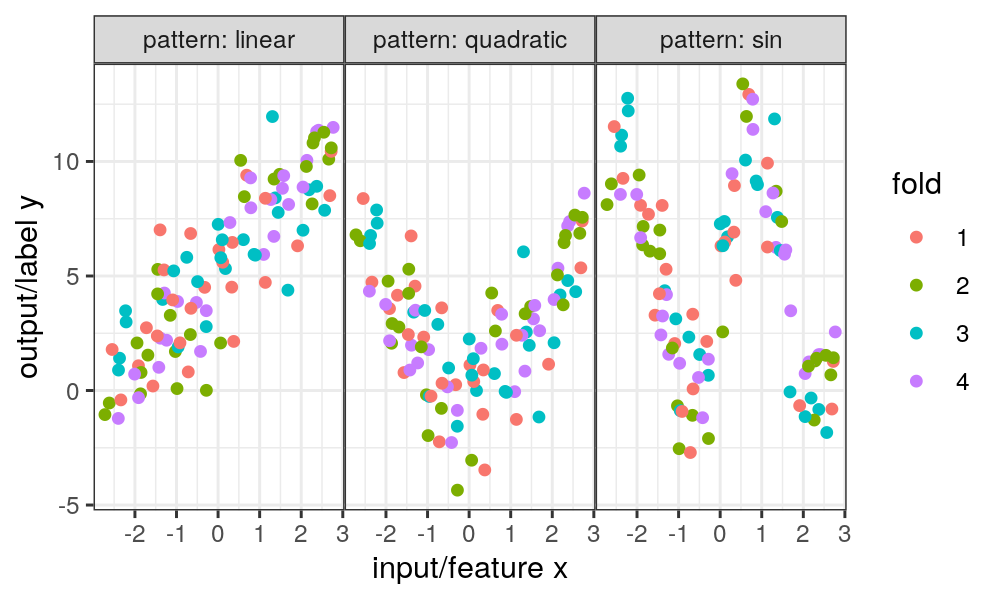
\includegraphics[width=\textwidth]{figure-overfitting-data-folds}
\end{frame}

\begin{frame}
  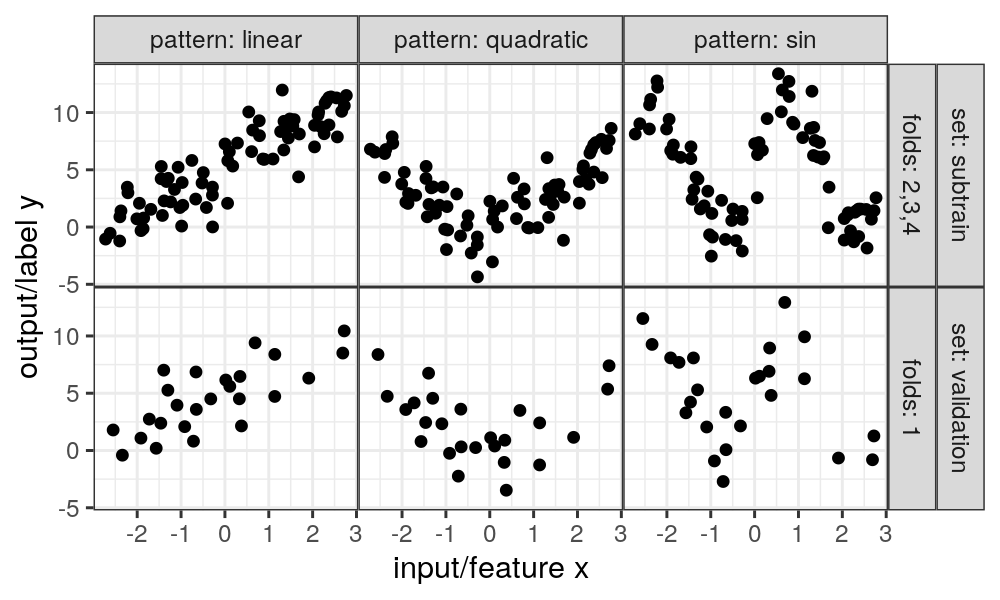
\includegraphics[width=\textwidth]{figure-overfitting-data-sets}
\end{frame}


\begin{frame}
  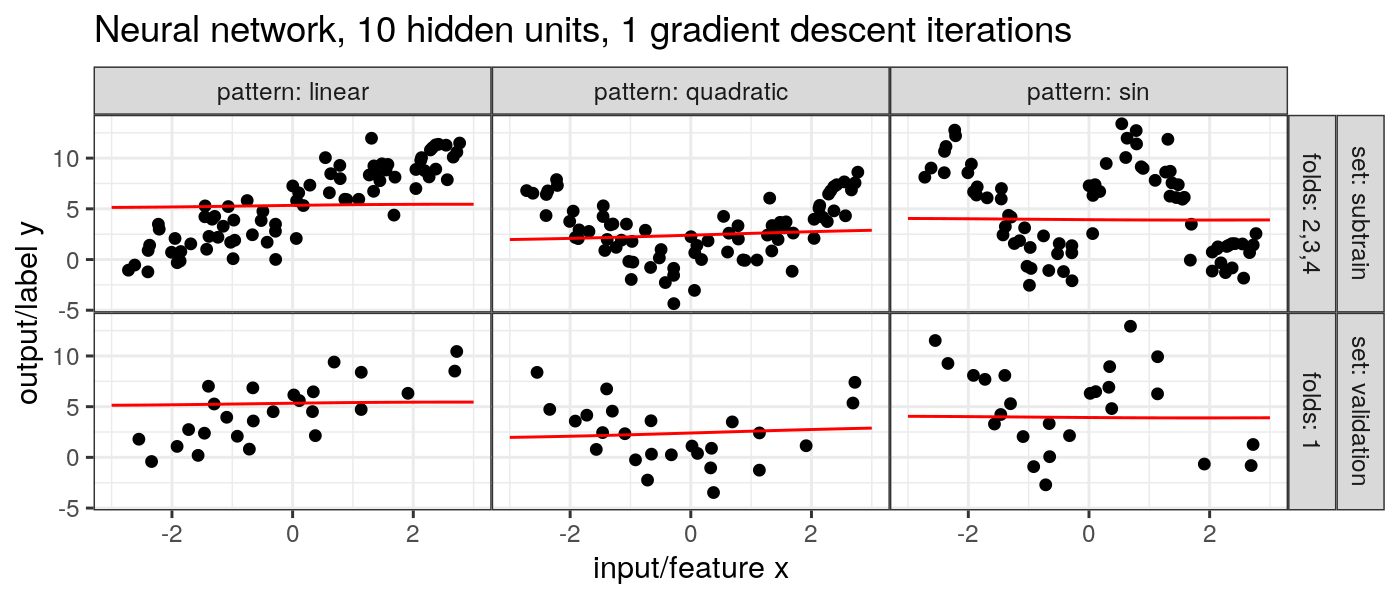
\includegraphics[width=\textwidth]{figure-overfitting-pred-units=10-maxit=1.png}
\end{frame}


\begin{frame}
  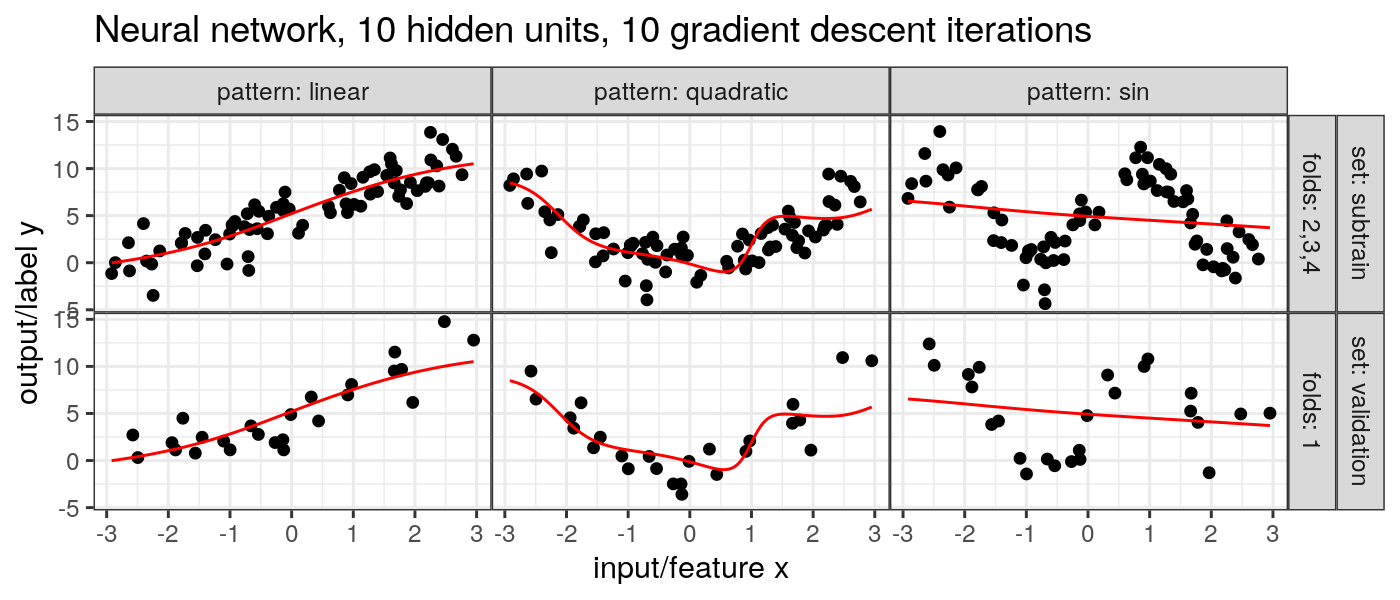
\includegraphics[width=\textwidth]{figure-overfitting-pred-units=10-maxit=10.png}
\end{frame}


\begin{frame}
  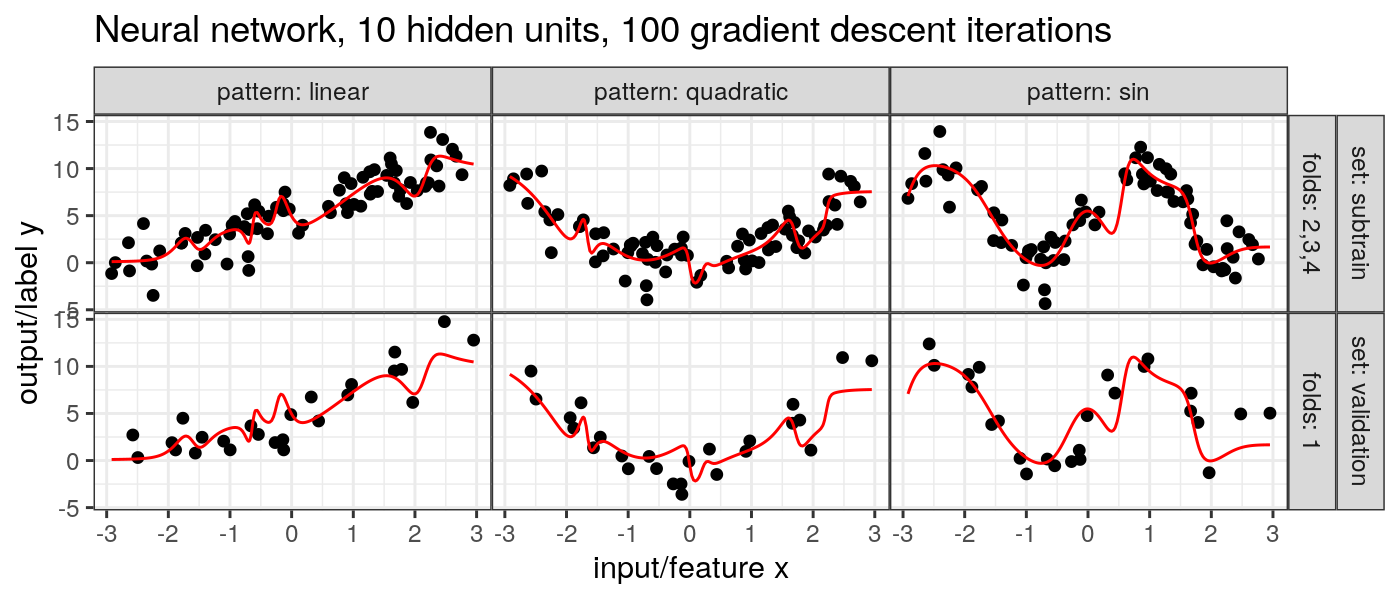
\includegraphics[width=\textwidth]{figure-overfitting-pred-units=10-maxit=100.png}
\end{frame}


\begin{frame}
  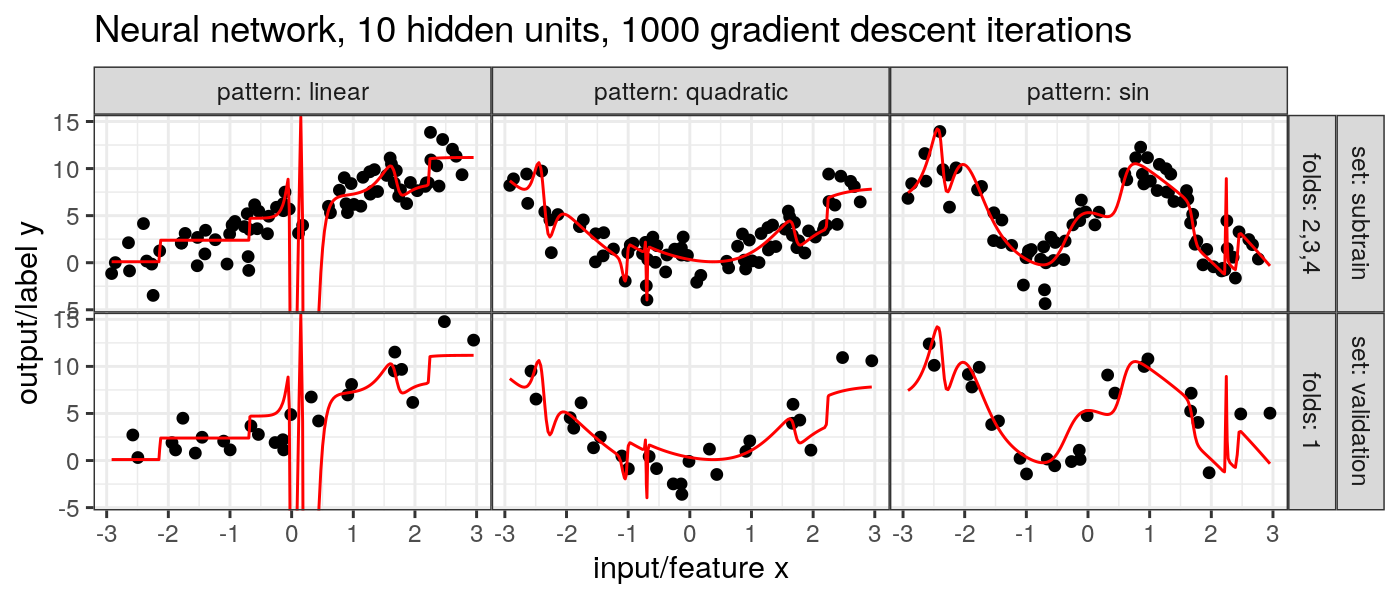
\includegraphics[width=\textwidth]{figure-overfitting-pred-units=10-maxit=1000.png}
\end{frame}


\begin{frame}
  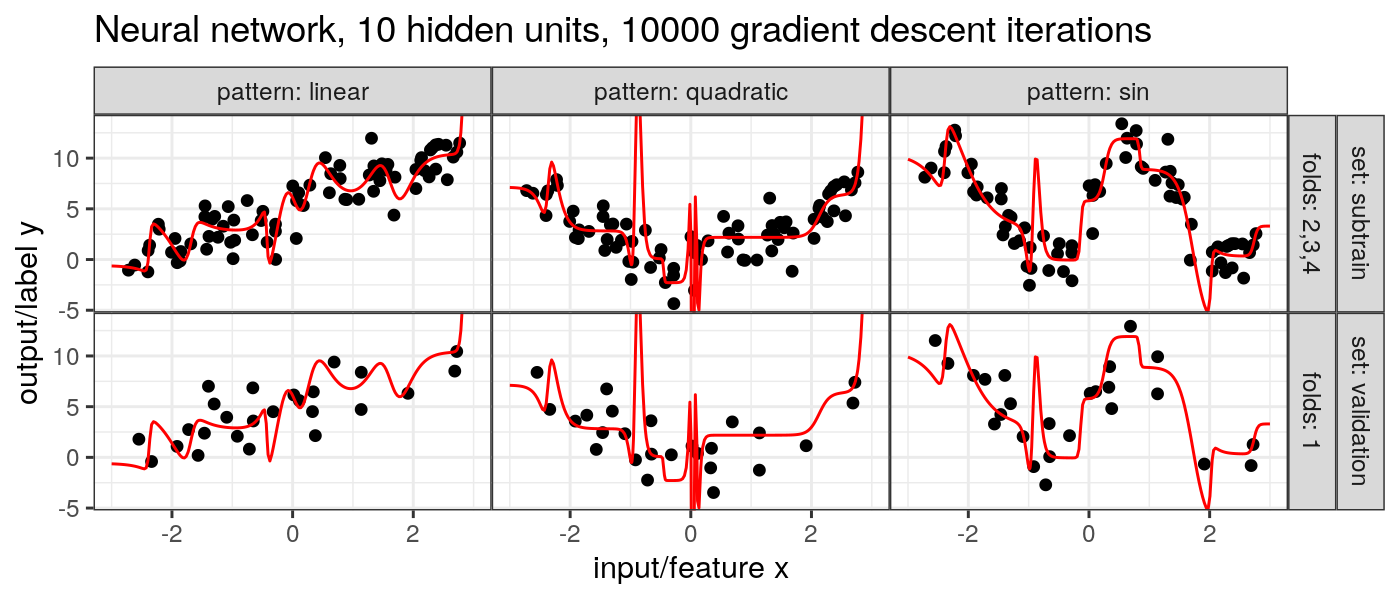
\includegraphics[width=\textwidth]{figure-overfitting-pred-units=10-maxit=10000.png}
\end{frame}


\begin{frame}
  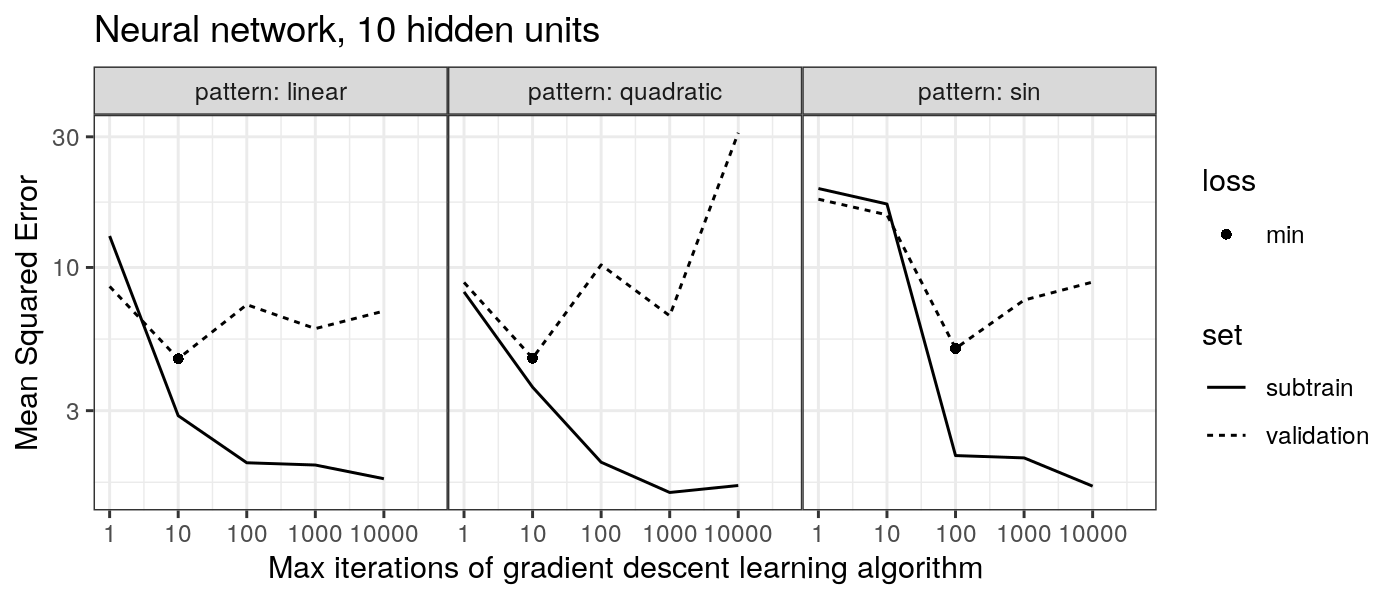
\includegraphics[width=\textwidth]{figure-overfitting-data-loss-10.png}
\end{frame}


\begin{frame}
  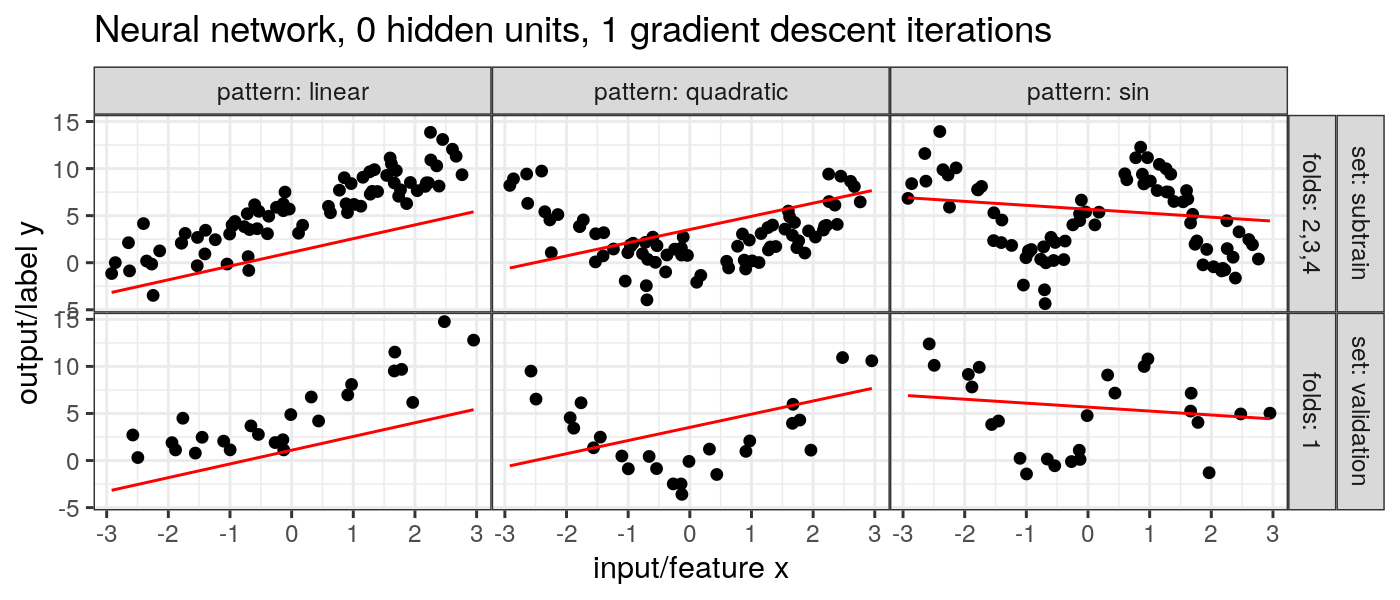
\includegraphics[width=\textwidth]{figure-overfitting-pred-units=0-maxit=1.png}
\end{frame}


\begin{frame}
  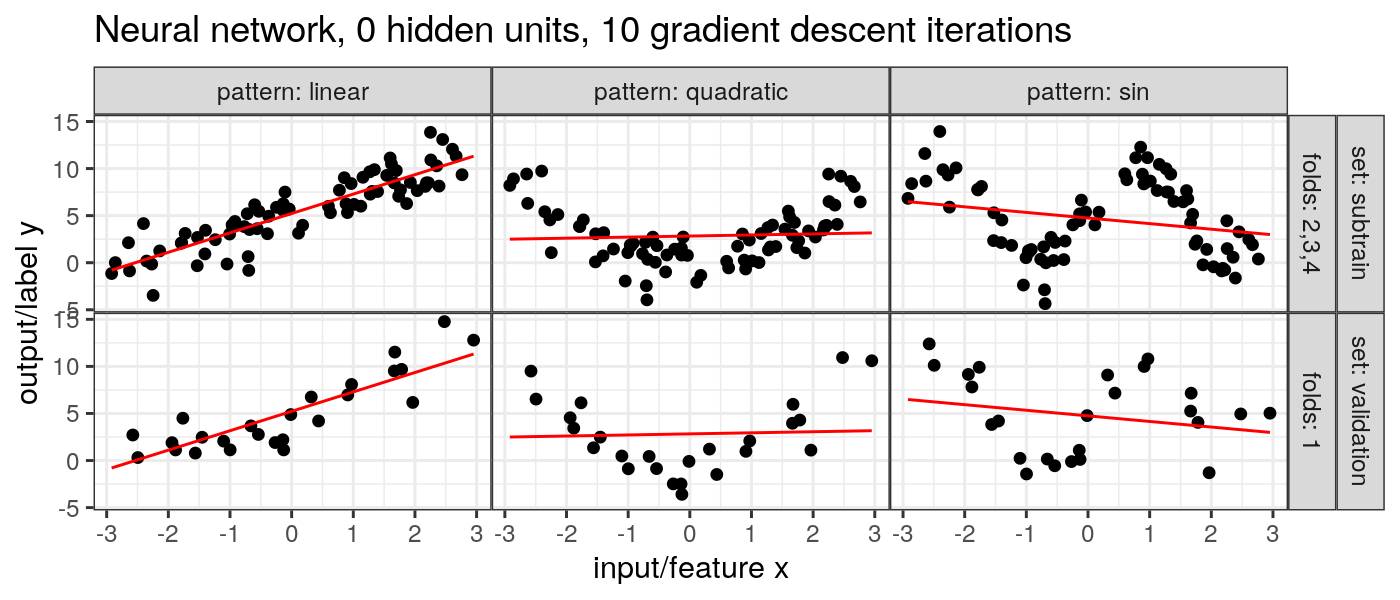
\includegraphics[width=\textwidth]{figure-overfitting-pred-units=0-maxit=10.png}
\end{frame}


\begin{frame}
  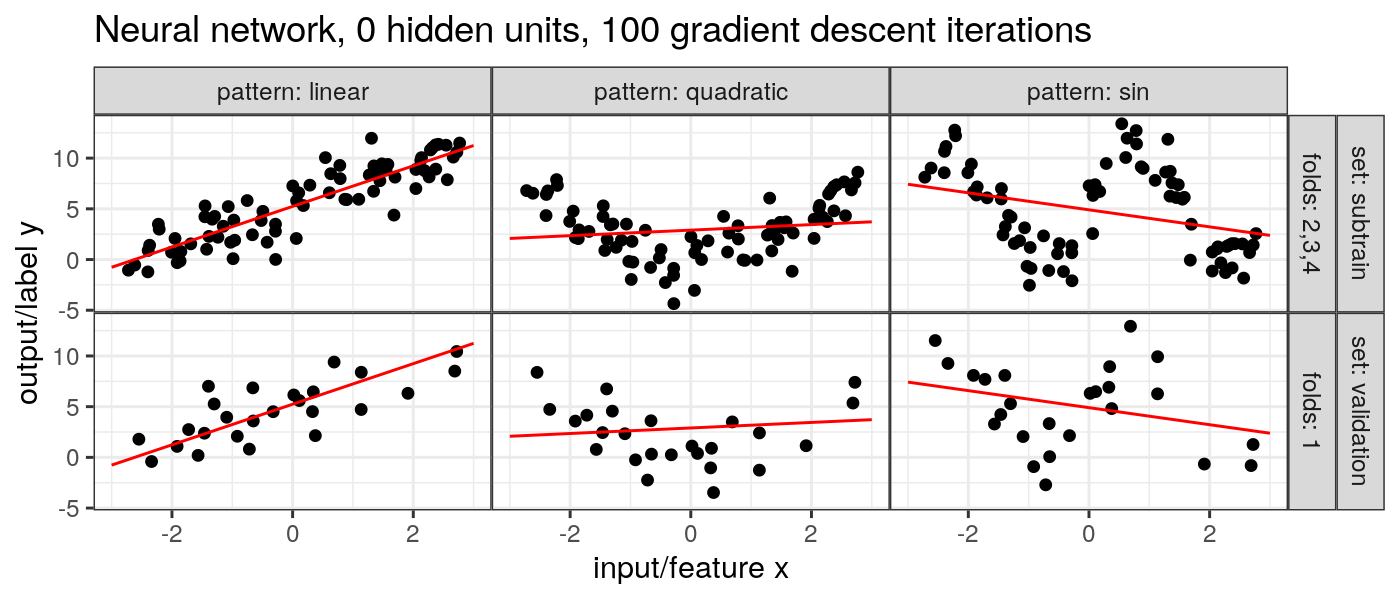
\includegraphics[width=\textwidth]{figure-overfitting-pred-units=0-maxit=100.png}
\end{frame}


\begin{frame}
  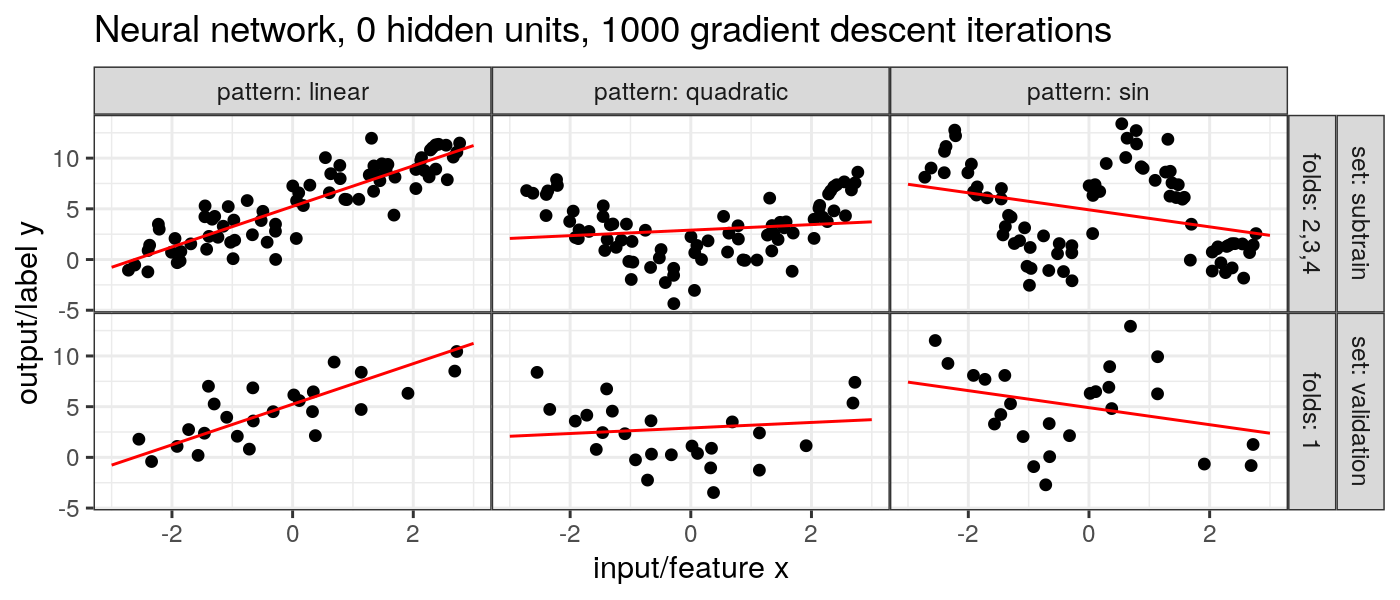
\includegraphics[width=\textwidth]{figure-overfitting-pred-units=0-maxit=1000.png}
\end{frame}


\begin{frame}
  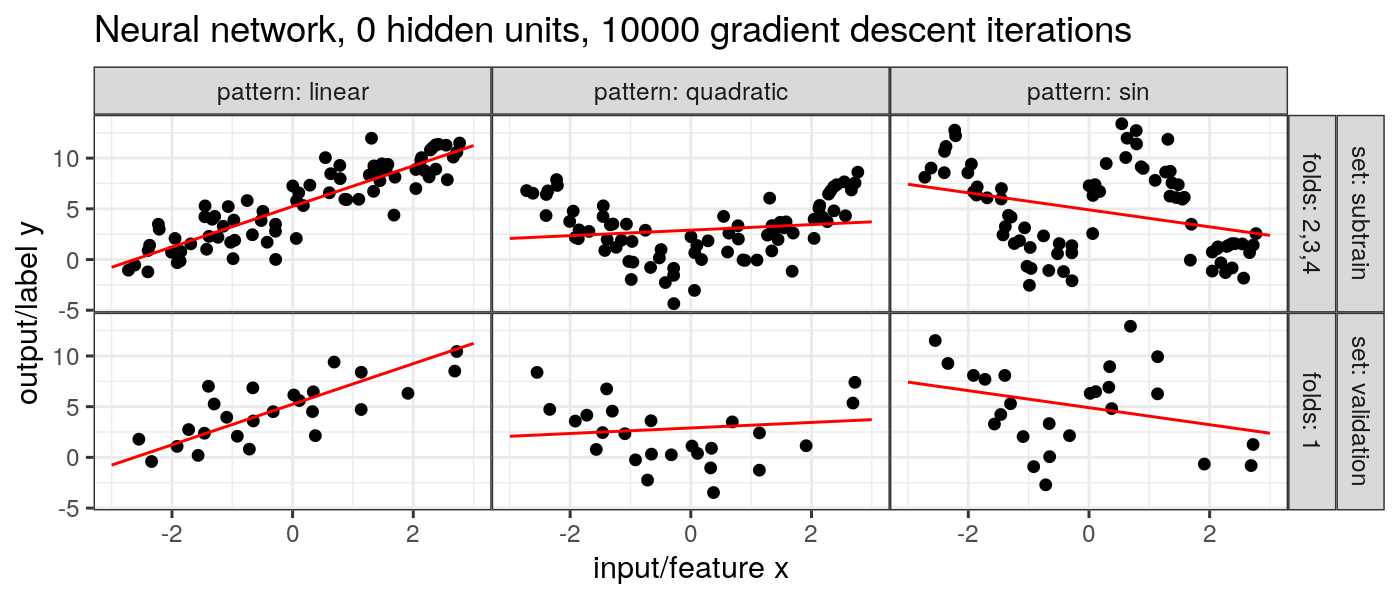
\includegraphics[width=\textwidth]{figure-overfitting-pred-units=0-maxit=10000.png}
\end{frame}


\begin{frame}
  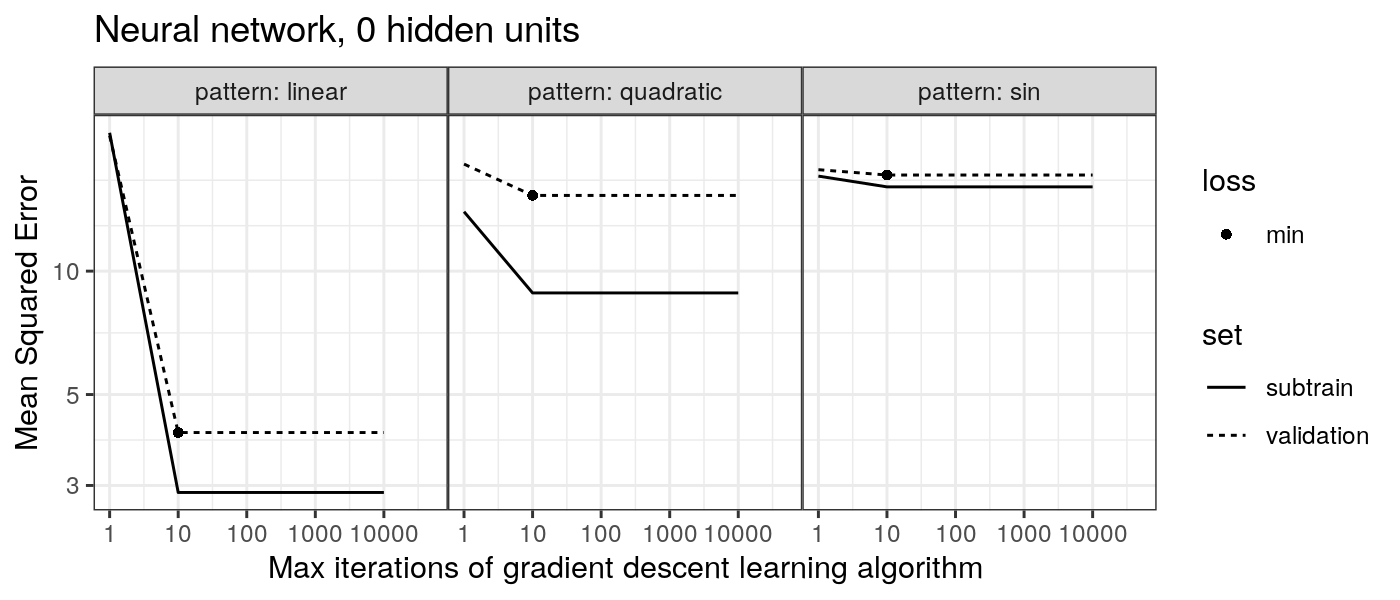
\includegraphics[width=\textwidth]{figure-overfitting-data-loss-0.png}
\end{frame}


\begin{frame}
  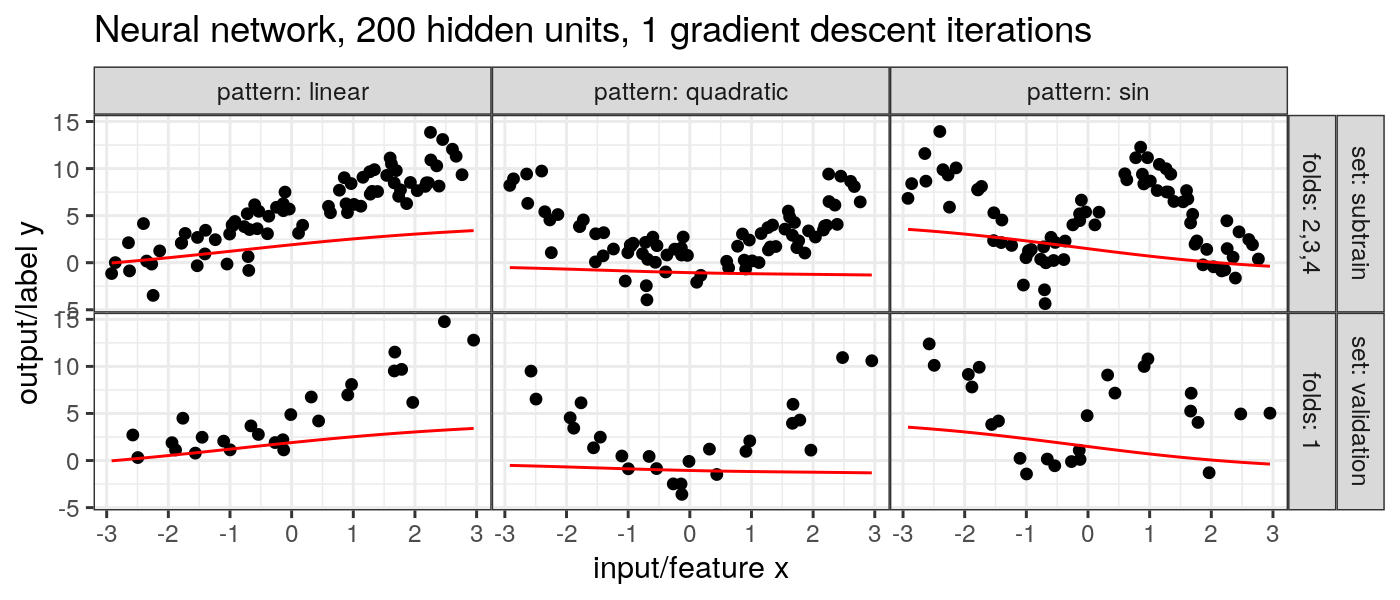
\includegraphics[width=\textwidth]{figure-overfitting-pred-units=200-maxit=1.png}
\end{frame}


\begin{frame}
  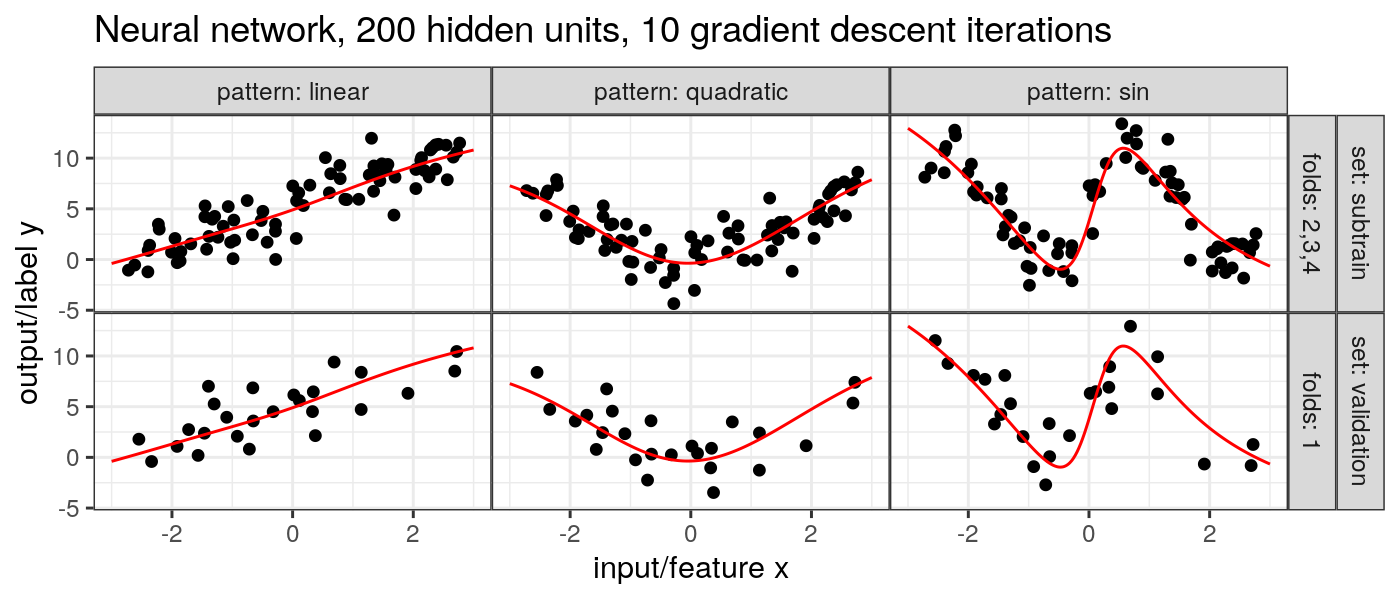
\includegraphics[width=\textwidth]{figure-overfitting-pred-units=200-maxit=10.png}
\end{frame}


\begin{frame}
  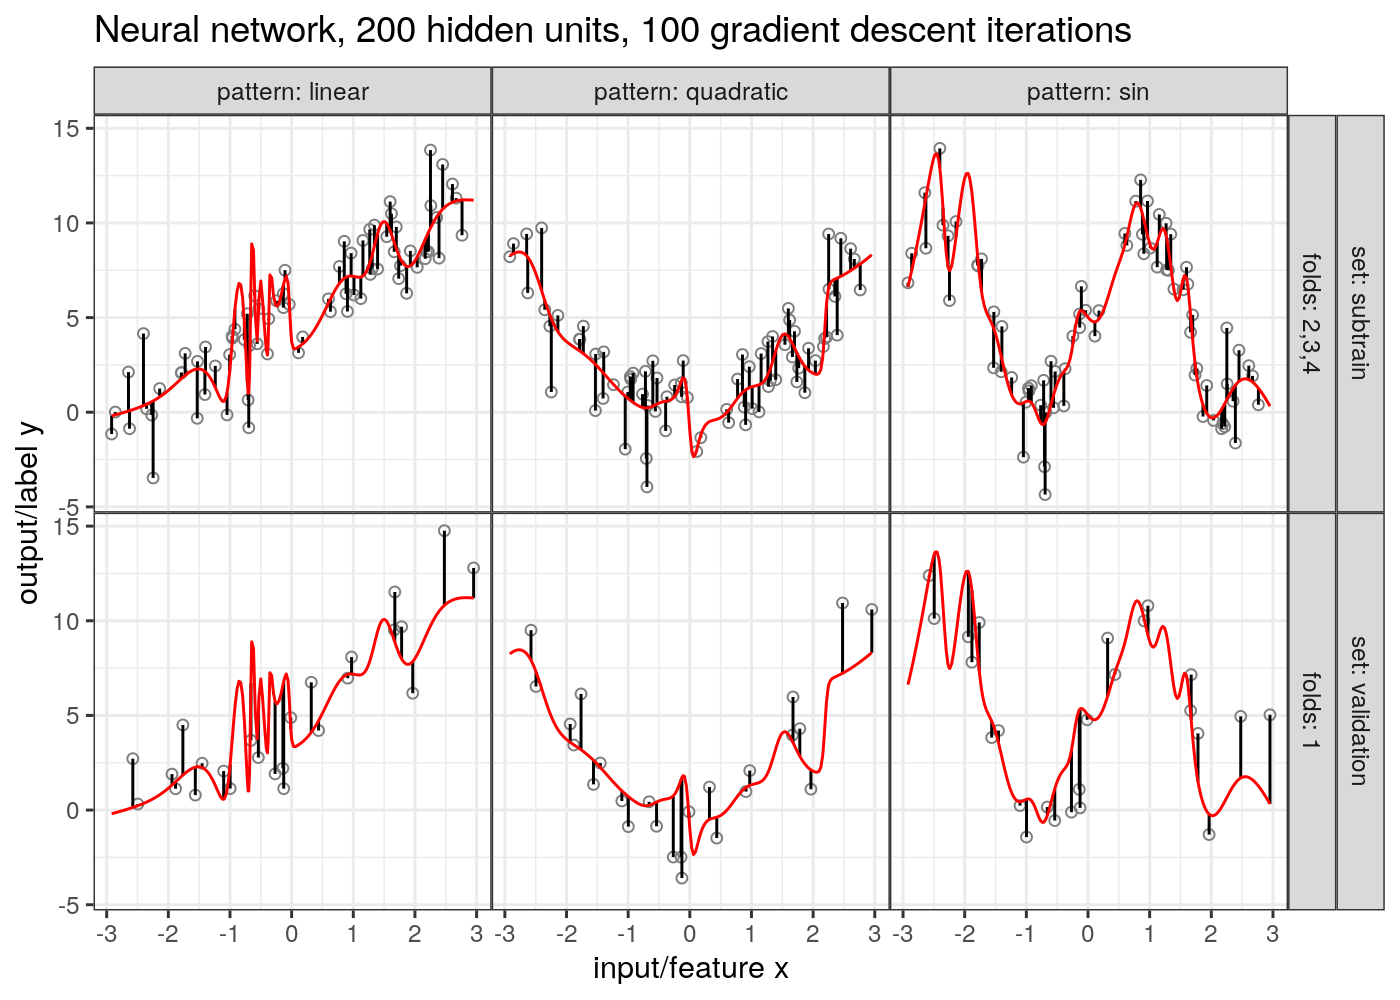
\includegraphics[width=\textwidth]{figure-overfitting-pred-units=200-maxit=100.png}
\end{frame}


\begin{frame}
  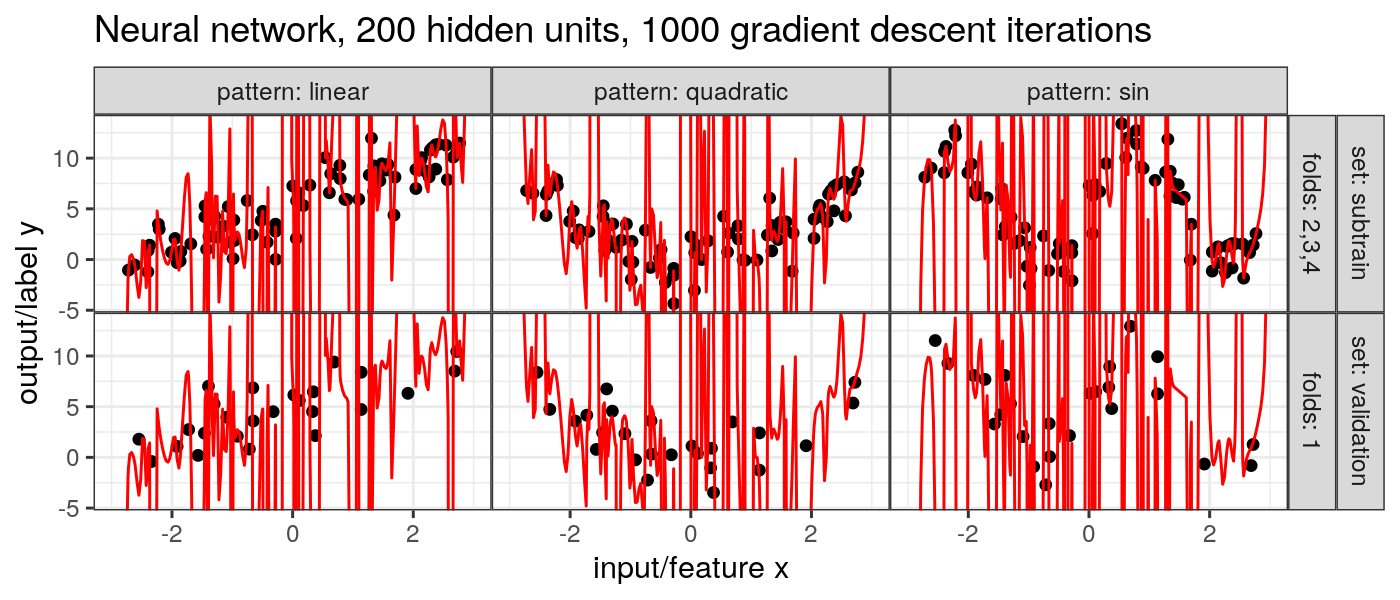
\includegraphics[width=\textwidth]{figure-overfitting-pred-units=200-maxit=1000.png}
\end{frame}


\begin{frame}
  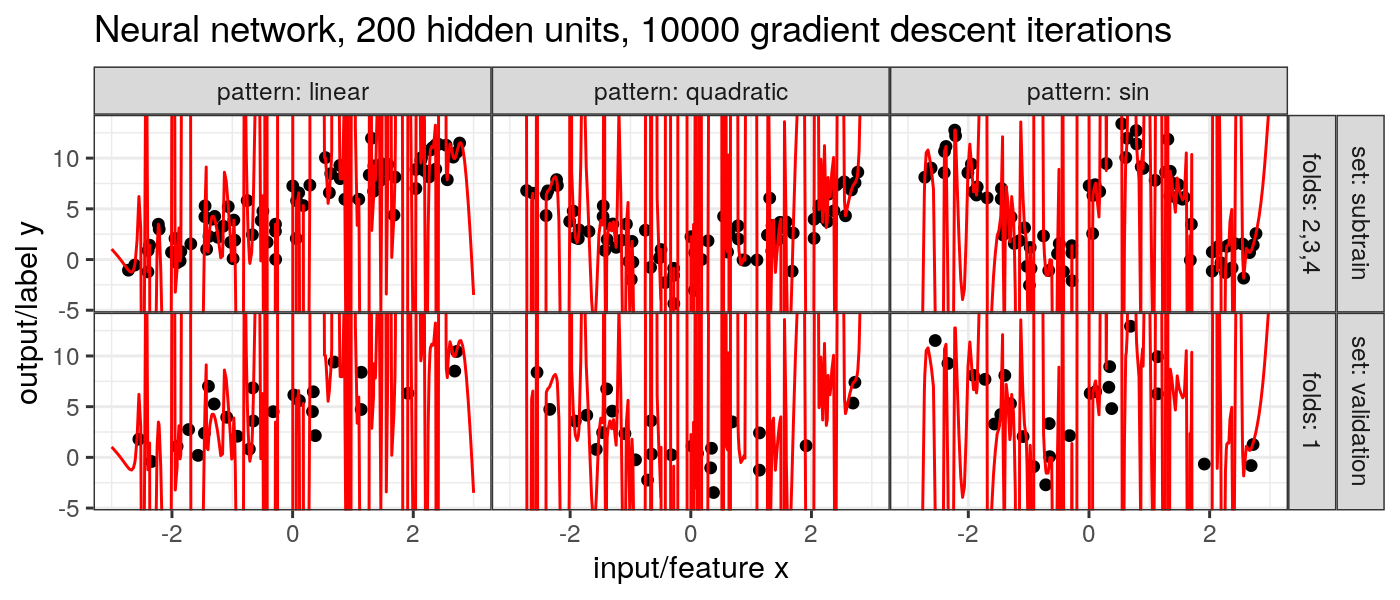
\includegraphics[width=\textwidth]{figure-overfitting-pred-units=200-maxit=10000.png}
\end{frame}


\begin{frame}
  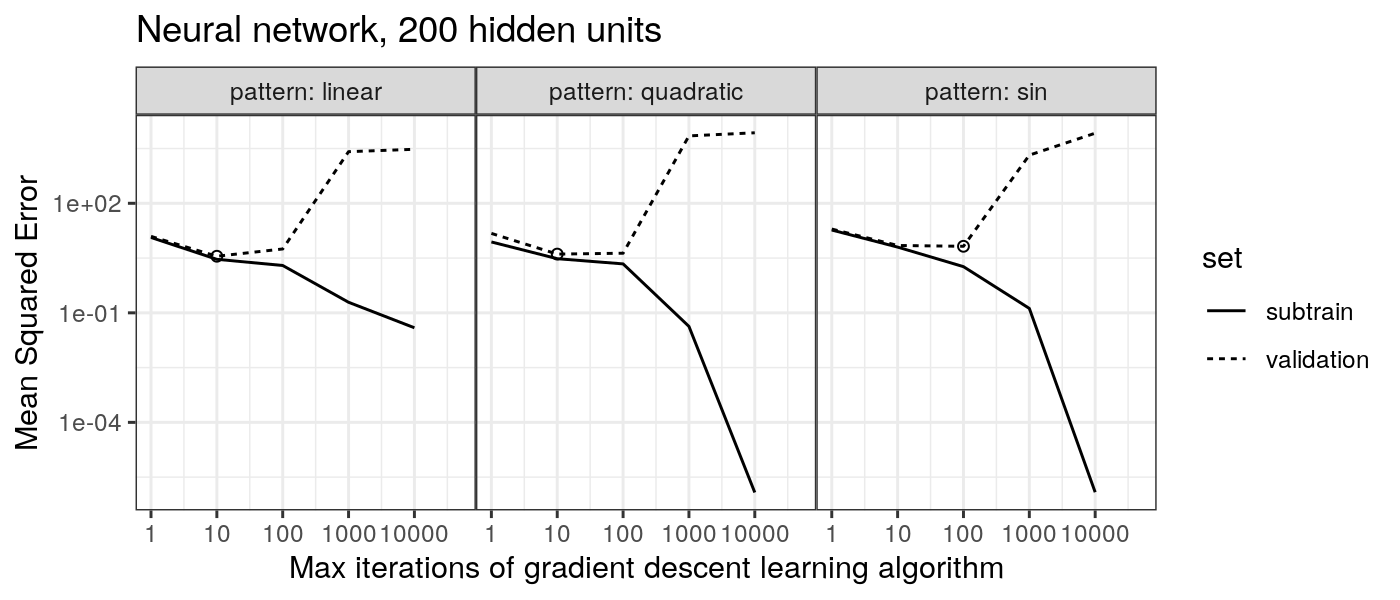
\includegraphics[width=\textwidth]{figure-overfitting-data-loss-200.png}
\end{frame}



\section{Classifying images of digits}

\begin{frame}
  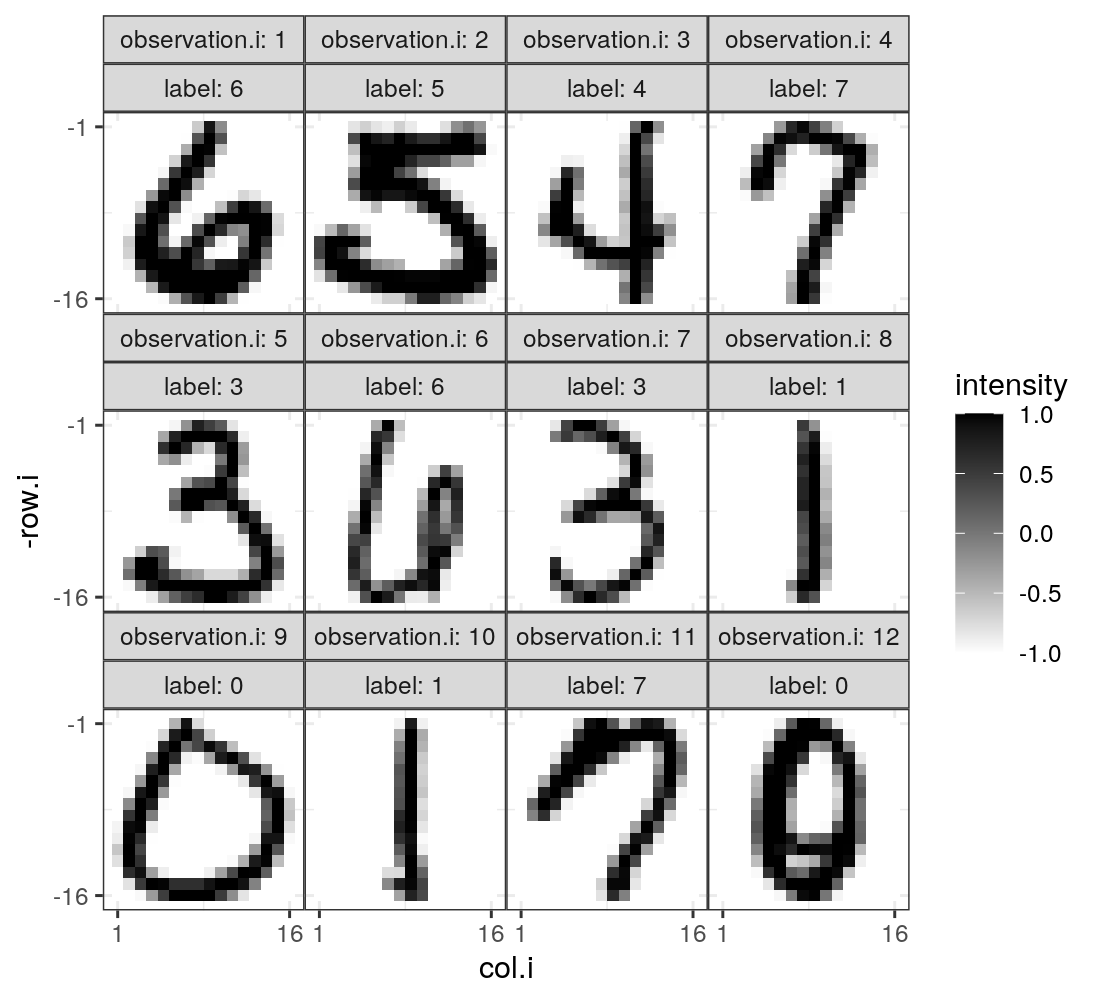
\includegraphics[width=\textwidth]{figure-validation-loss-digits}
\end{frame}

\begin{frame}[fragile]
  \frametitle{Representation of digits in CSV}

  \begin{itemize}
  \item Each image is one row.
  \item First row is output/label/class to predict.
  \item Other 256 columns are pixel intensity values.
  \end{itemize}

\begin{verbatim}
 1:  6 -1 -1  ... -1.000 -1.000   -1
 2:  5 -1 -1  ... -0.671 -0.828   -1
 3:  4 -1 -1  ... -1.000 -1.000   -1
 4:  7 -1 -1  ... -1.000 -1.000   -1
 5:  3 -1 -1  ... -0.883 -1.000   -1
 6:  6 -1 -1  ... -1.000 -1.000   -1
 7:  3 -1 -1  ... -1.000 -1.000   -1
 8:  1 -1 -1  ... -1.000 -1.000   -1
 9:  0 -1 -1  ... -1.000 -1.000   -1
10:  1 -1 -1  ... -1.000 -1.000   -1
11:  7 -1 -1  ... -1.000 -1.000   -1
12:  0 -1 -1  ... -1.000 -1.000   -1
\end{verbatim}
  
\end{frame}

\begin{frame}[fragile]
  \frametitle{Converting label column to matrix for neural network}

  This is a ``one hot'' encoding of the class labels.
  
\begin{verbatim}
zip.dt <- data.table::fread("zip.gz")
zip.y.mat <- keras::to_categorical(zip.dt$V1)

      0 1 2 3 4 5 6 7 8 9
 [1,] 0 0 0 0 0 0 1 0 0 0
 [2,] 0 0 0 0 0 1 0 0 0 0
 [3,] 0 0 0 0 1 0 0 0 0 0
 [4,] 0 0 0 0 0 0 0 1 0 0
 [5,] 0 0 0 1 0 0 0 0 0 0
 [6,] 0 0 0 0 0 0 1 0 0 0
 [7,] 0 0 0 1 0 0 0 0 0 0
 [8,] 0 1 0 0 0 0 0 0 0 0
 [9,] 1 0 0 0 0 0 0 0 0 0
[10,] 0 1 0 0 0 0 0 0 0 0
[11,] 0 0 0 0 0 0 0 1 0 0
[12,] 1 0 0 0 0 0 0 0 0 0
\end{verbatim}


\end{frame}

\begin{frame}[fragile]
  \frametitle{Conversion to array for input to neural network}
Use array function with all columns except first as data.  
\begin{verbatim}
zip.size <- 16
zip.X.array <- array(
  data = unlist(zip.dt[1:nrow(zip.dt),-1]),
  dim = c(nrow(zip.dt), zip.size, zip.size, 1))
\end{verbatim}
Need to specify dimensions of array:
\begin{itemize}
\item Observations: same as the number of rows in the CSV table.
\item Pixels wide: 16.
\item Pixels high: 16.
\item Channels: 1 (greyscale image).
\end{itemize}

\end{frame}

\begin{frame}[fragile]
  \frametitle{Linear model R code}

\begin{verbatim}
library(keras)
linear.model <- keras_model_sequential() %>%
  layer_flatten(
    input_shape = dim(zip.X.array)[-1]) %>%
  layer_dense(
    units = ncol(zip.y.mat),
    activation = 'softmax')
\end{verbatim}

\end{frame}
 
\begin{frame}
  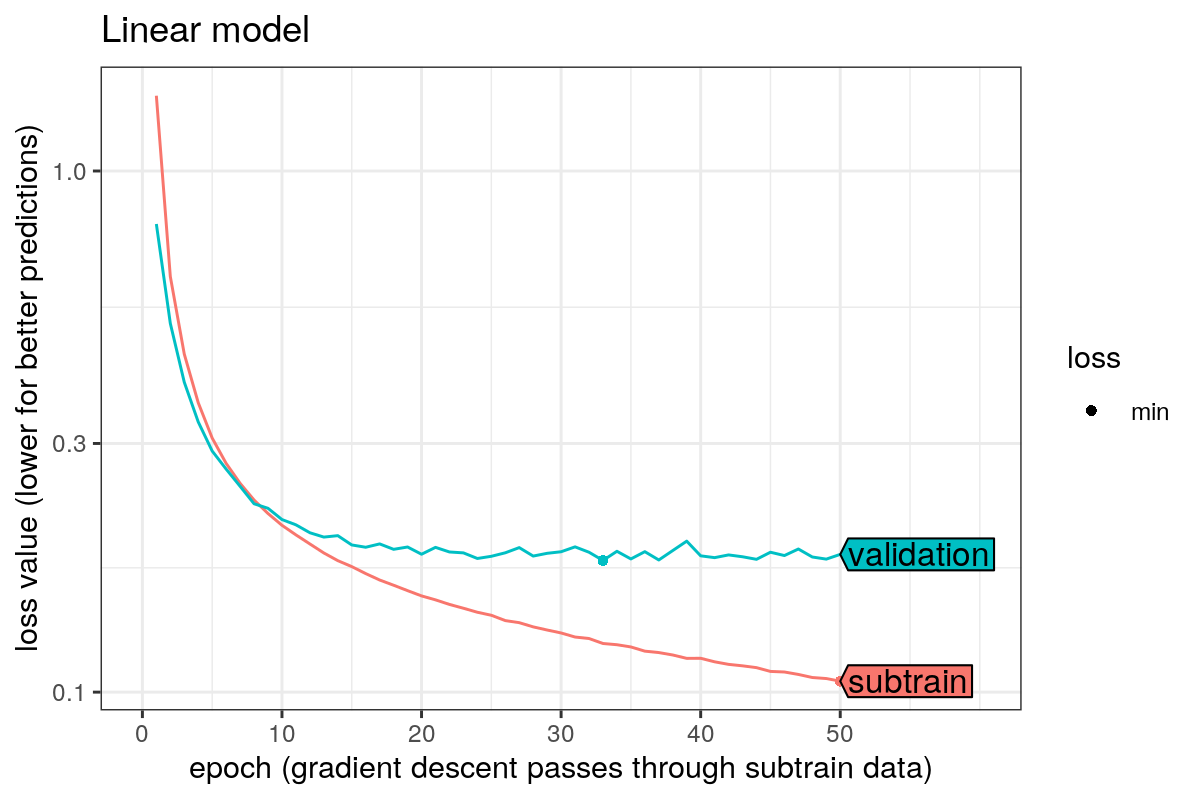
\includegraphics[width=\textwidth]{figure-validation-loss-linear}
\end{frame}
 
\begin{frame}[fragile]
  \frametitle{Convolutional model R code}

\begin{verbatim}
library(keras)
conv.model <- keras_model_sequential() %>%
  layer_conv_2d(
    input_shape = dim(zip.X.array)[-1],
    filters = 20,
    kernel_size = c(3,3),
    activation = 'relu') %>% 
  layer_max_pooling_2d(pool_size = c(2, 2)) %>%
  layer_flatten() %>%
  layer_dense(units = 100, activation = 'relu') %>% 
  layer_dense(
    units = ncol(zip.y.mat), 
    activation = 'softmax')
\end{verbatim}

\end{frame}
 
\begin{frame}
  \includegraphics[width=\textwidth]{figure-validation-loss-conv}
\end{frame}
 
\begin{frame}[fragile]
  \frametitle{Dense (fully connected) neural network R code}

\begin{verbatim}
library(keras)
dense.model <- keras_model_sequential() %>%
  layer_flatten(
    input_shape = dim(zip.X.array)[-1]) %>%
  layer_dense(units = 100, activation = 'relu') %>% 
  layer_dense(units = 100, activation = 'relu') %>% 
  layer_dense(units = 100, activation = 'relu') %>% 
  layer_dense(units = 100, activation = 'relu') %>%
  layer_dense(units = 100, activation = 'relu') %>%
  layer_dense(units = 100, activation = 'relu') %>% 
  layer_dense(units = 100, activation = 'relu') %>%   
  layer_dense(units = 100, activation = 'relu') %>% 
  layer_dense(
    units = ncol(zip.y.mat), 
    activation = 'softmax')
\end{verbatim}

\end{frame}
 
\begin{frame}
  \includegraphics[width=\textwidth]{figure-validation-loss-dense}
\end{frame}
 
\begin{frame}
  \includegraphics[width=\textwidth]{figure-validation-loss-three}
\end{frame}
 
\begin{frame}
  \includegraphics[width=\textwidth]{figure-test-accuracy-baseline}
\end{frame}
 
\begin{frame}
  \includegraphics[width=\textwidth]{figure-test-accuracy}
\end{frame}
 
\end{document}
